\section*{Exercise 1}
Suppose that we wish to use the Gibbs sampler on
\begin{equation*}
\pi (x, y) \propto \exp \left(-\frac{1}{2}(x - 1)^2(y - 2)^2\right).
\end{equation*}

\begin{enumerate}
\item Write down the two ``full'' conditional distributions associated to $\pi (x, y)$.
\item Does the resulting Gibbs sampler make any sense?
\end{enumerate}

\section*{Solution}

Given the target distribution:
\begin{equation*}
\pi (x, y) \propto \exp \left(-\frac{1}{2}(x - 1)^2(y - 2)^2\right)
\end{equation*}

\subsection*{Question 1: Full conditional distributions}

To find the full conditional distributions, we examine the distribution of each variable while treating the other as fixed.

\textbf{Conditional distribution of $X$ given $Y$:}

\begin{align*}
\pi(x|y) &\propto \exp \left(-\frac{1}{2}(x - 1)^2(y - 2)^2\right)\\
&\propto \exp \left(-\frac{(y - 2)^2}{2}(x - 1)^2\right)
\end{align*}

Since $(y-2)^2$ is constant when $y$ is fixed, this is the kernel of a normal distribution with mean 1 and precision $(y-2)^2$. Therefore:

\begin{equation*}
\pi(x|y) = \mathcal{N}\left(1, \frac{1}{(y-2)^2}\right) \text{ for } y \neq 2
\end{equation*}

\textbf{Conditional distribution of $Y$ given $X$:}

Similarly, we have:

\begin{equation*}
\pi(y|x) = \mathcal{N}\left(2, \frac{1}{(x-1)^2}\right) \text{ for } x \neq 1
\end{equation*}

\subsection*{Part 2: Does the Gibbs sampler make sense?}

\textbf{Answer: No, the Gibbs sampler does NOT make sense for this distribution.}

Here are the fundamental problems:

\paragraph{1. Undefined conditional distributions:}
\begin{itemize}
\item When $y = 2$: $\text{Var}(X|y=2) = \frac{1}{(2-2)^2} = \frac{1}{0} = \infty$ (undefined)
\item When $x = 1$: $\text{Var}(Y|x=1) = \frac{1}{(1-1)^2} = \frac{1}{0} = \infty$ (undefined)
\end{itemize}

\paragraph{2. Improper joint distribution:}
The joint distribution $\pi(x,y) \propto \exp\left(-\frac{1}{2}(x-1)^2(y-2)^2\right)$ becomes constant along the lines $x = 1$ and $y = 2$:
\begin{itemize}
\item Along $x = 1$: $\pi(1,y) \propto \exp(0) = 1$ (constant for all $y$)
\item Along $y = 2$: $\pi(x,2) \propto \exp(0) = 1$ (constant for all $x$)
\end{itemize}

This means the distribution does not integrate to a finite value, making it an improper distribution.

\paragraph{3. Practical failure:}
\begin{itemize}
\item If the sampler reaches exactly $x = 1$ or $y = 2$, the corresponding conditional distribution becomes improper (uniform over the entire real line), making sampling impossible.
\item Even near these values, the conditional variances become extremely large, leading to poor mixing and numerical instability.
\item The sampler would exhibit erratic behavior and fail to converge to a proper stationary distribution.
\end{itemize}

\paragraph{Conclusion:}
The Gibbs sampler fails because the target distribution is improper and the conditional distributions are not well-defined at the modal lines. This example illustrates the importance of verifying that the target distribution is proper before attempting to use MCMC methods.

\begin{figure}[h!]
    \centering
    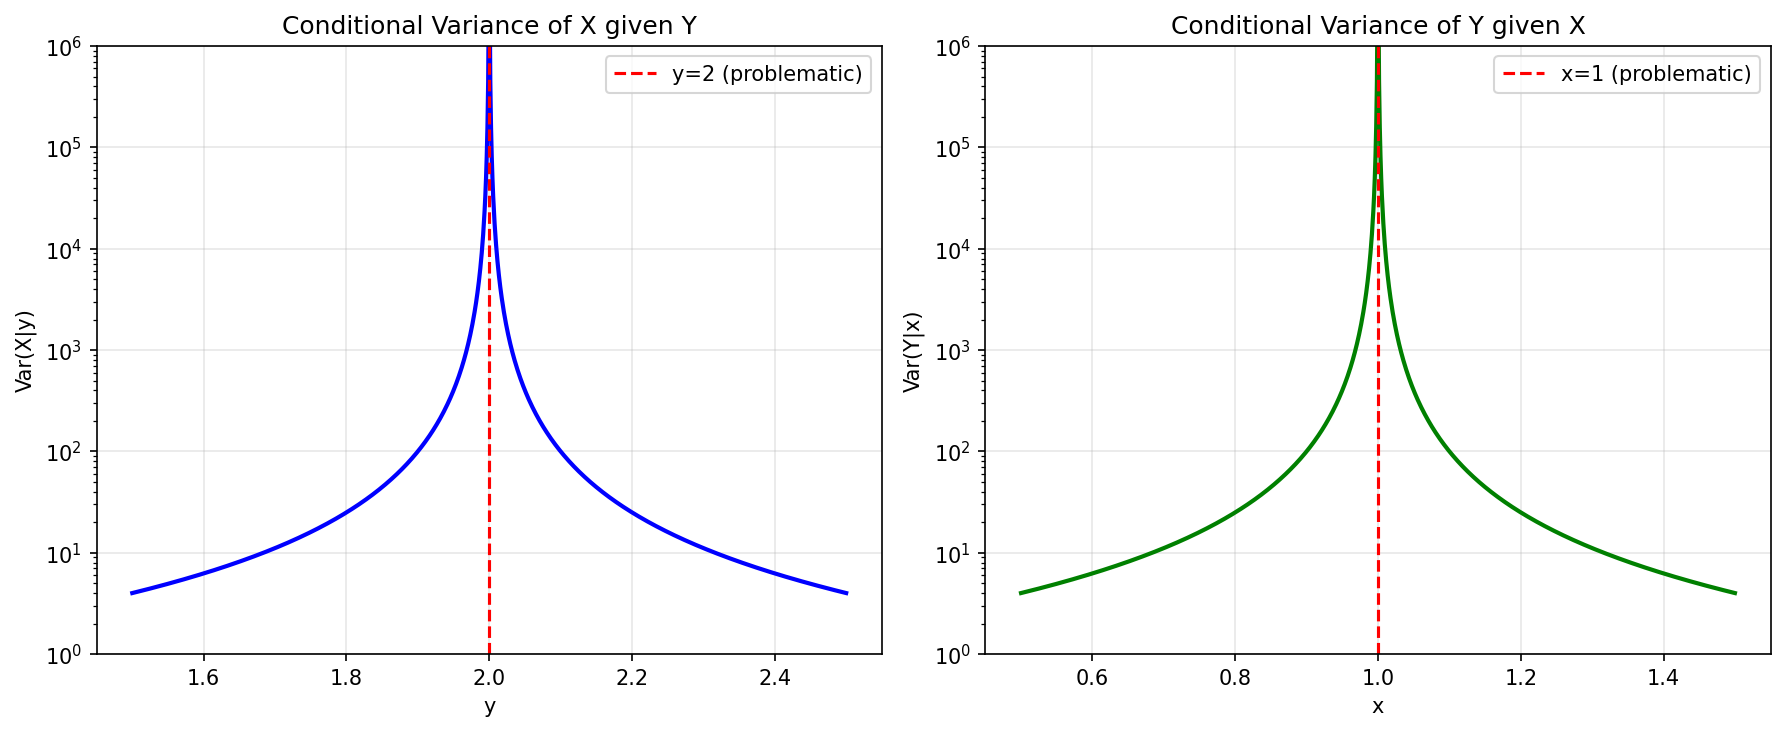
\includegraphics[width=0.95\textwidth]{exercise1_conditional_variances.png}
    \caption{Plot of the conditional variances $\text{Var}(X|Y)$ and $\text{Var}(Y|X)$ showing they become infinite at $y=2$ and $x=1$ respectively.}
    \label{fig:exercise1}
\end{figure}    